        \documentclass[crop,tikz, border=5pt]{beamer}
        
        \usepackage{tikz}
        \usetikzlibrary{calc}
        \usetheme{default}
        \usefonttheme{professionalfonts}
        \setbeamertemplate{navigation symbols}{}
        \setbeamerfont{frametitle}{series=\bfseries}
        \tikzset{ n/.style = { circle % node
        , very thick
        , draw
        , fill = yellow
        , minimum size = 4mm
        }
        , d/.style = { rectangle % distance
        , minimum size = 4mm
        , font = \color{blue!50!black}\LARGE
        }
        , v/.style = { rectangle % via vertex
        , minimum size = 4mm
        , font = \color{green!50!black}
        }
        }
        \newcommand{\oo}{\ensuremath\infty}
        \def\dst(#1,#2)#3{% distance
        \pgfmathtruncatemacro{\x}{3*#2}
        \pgfmathtruncatemacro{\y}{(-2)*#1+12}
        \node[d] at (\x,\y) {#3};
        }
        \def\via(#1,#2)#3{% via vertex
        \pgfmathtruncatemacro{\x}{3*#2+1}
        \pgfmathtruncatemacro{\y}{(-2)*#1+12}
        \node[v] at (\x,\y) {#3};
        }
    
        \begin{document}
        
        \begin{frame}
        \frametitle{Bellman-Ford Algorithm : Input}
        \begin{center}
        
        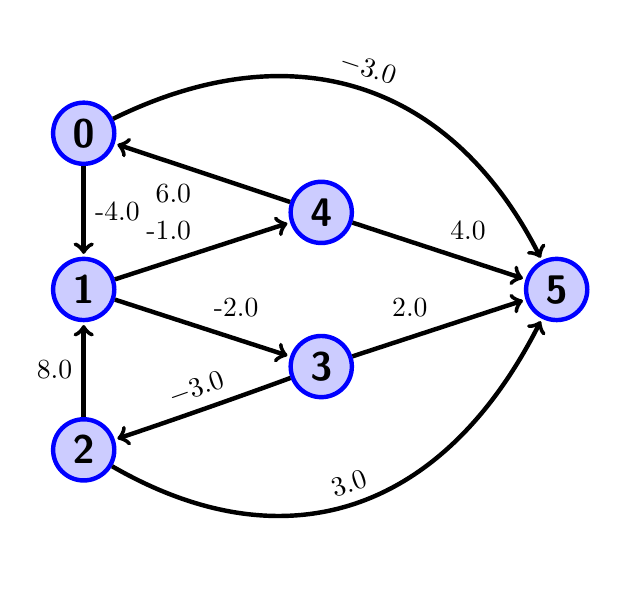
\begin{tikzpicture}[shorten >=1pt, auto, node distance=3cm, ultra thick,
        node_style/.style={circle,draw=blue,fill=blue!20!,font=\sffamily\Large\bfseries},
        edge_node_style/.style={draw=none,fill=none,midway,sloped},
        selected_node_style/.style={circle,draw=blue,fill=yellow!20!,font=\sffamily\Large\bfseries},
        edge_style/.style={draw=black, ultra thick,->},
        selected_edge_style/.style={draw=yellow, ultra thick,->}]
        \tikzset{quadratic bezier/.style={ to path={(\tikztostart) .. controls($#1!1/3!(\tikztostart)$) and ($#1!1/3!(\tikztotarget)$).. (\tikztotarget)}}}
        
        \node [node_style,label={[text=blue]10:$$}](n1) at (3.471,-1.527) {0};
        \node [node_style,label={[text=blue]10:$$}](n2) at (3.471,-3.511) {1};
        \node [node_style,label={[text=blue]10:$$}](n3) at (3.471,-5.548) {2};
        \node [node_style,label={[text=blue]10:$$}](n4) at (6.488,-4.49) {3};
        \node [node_style,label={[text=blue]10:$$}](n5) at (6.488,-2.532) {4};
        \node [node_style,label={[text=blue]10:$$}](n6) at (9.478,-3.511) {5};\draw [edge_style] (n2) to[edge label=-1.0] (n5);
            \coordinate (crtl2)  at (7.473,0.442);
                        \draw [edge_style] (n1) .. controls($(crtl2)!1/3!(n1)$) and ($(crtl2)!1/3!(n6)$).. node [edge_node_style] {$-3.0$} (n6);
                    \coordinate (crtl3)  at (7.324,-7.771);
                        \draw [edge_style] (n3) .. controls($(crtl3)!1/3!(n3)$) and ($(crtl3)!1/3!(n6)$).. node [edge_node_style] {$3.0$} (n6);
                    \coordinate (crtl4)  at (5.003,-5.039);
                        \draw [edge_style] (n4) .. controls($(crtl4)!1/3!(n4)$) and ($(crtl4)!1/3!(n3)$).. node [edge_node_style] {$-3.0$} (n3);
                    \draw [edge_style] (n5) to[edge label=4.0] (n6);
            \draw [edge_style] (n5) to[edge label=6.0] (n1);
            \draw [edge_style] (n2) to[edge label=-2.0] (n4);
            \draw [edge_style] (n4) to[edge label=2.0] (n6);
            \draw [edge_style] (n3) to[edge label=8.0] (n2);
            \draw [edge_style] (n1) to[edge label=-4.0] (n2);
            
        \end{tikzpicture}
    
        \end{center}
        \end{frame}
        
            \begin{frame}
            \frametitle{Bellman-Ford Algorithm : Iteration 1 }
            \begin{center}
            
        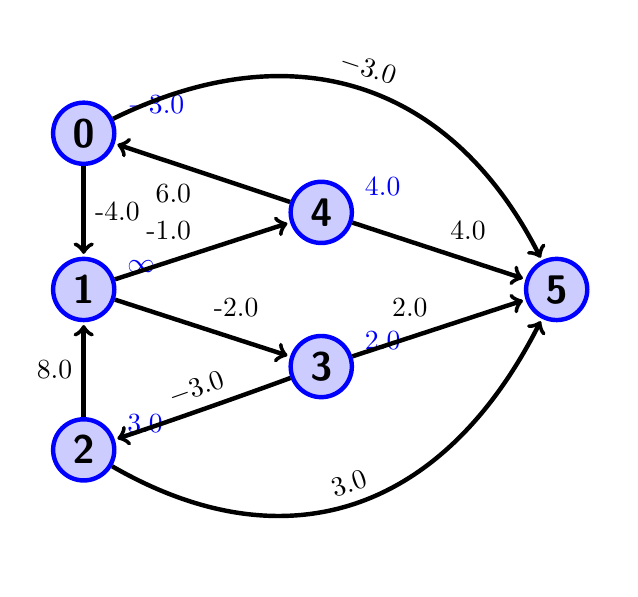
\begin{tikzpicture}[shorten >=1pt, auto, node distance=3cm, ultra thick,
        node_style/.style={circle,draw=blue,fill=blue!20!,font=\sffamily\Large\bfseries},
        edge_node_style/.style={draw=none,fill=none,midway,sloped},
        selected_node_style/.style={circle,draw=blue,fill=yellow!20!,font=\sffamily\Large\bfseries},
        edge_style/.style={draw=black, ultra thick,->},
        selected_edge_style/.style={draw=yellow, ultra thick,->}]
        \tikzset{quadratic bezier/.style={ to path={(\tikztostart) .. controls($#1!1/3!(\tikztostart)$) and ($#1!1/3!(\tikztotarget)$).. (\tikztotarget)}}}
        
        \node [node_style,label={[text=blue]10:$-3.0$}](n1) at (3.471,-1.527) {0};
        \node [node_style,label={[text=blue]10:$\infty$}](n2) at (3.471,-3.511) {1};
        \node [node_style,label={[text=blue]10:$3.0$}](n3) at (3.471,-5.548) {2};
        \node [node_style,label={[text=blue]10:$2.0$}](n4) at (6.488,-4.49) {3};
        \node [node_style,label={[text=blue]10:$4.0$}](n5) at (6.488,-2.532) {4};
        \node [node_style,label={[text=blue]10:$$}](n6) at (9.478,-3.511) {5};\draw [edge_style] (n2) to[edge label=-1.0] (n5);
            \coordinate (crtl2)  at (7.473,0.442);
                        \draw [edge_style] (n1) .. controls($(crtl2)!1/3!(n1)$) and ($(crtl2)!1/3!(n6)$).. node [edge_node_style] {$-3.0$} (n6);
                    \coordinate (crtl3)  at (7.324,-7.771);
                        \draw [edge_style] (n3) .. controls($(crtl3)!1/3!(n3)$) and ($(crtl3)!1/3!(n6)$).. node [edge_node_style] {$3.0$} (n6);
                    \coordinate (crtl4)  at (5.003,-5.039);
                        \draw [edge_style] (n4) .. controls($(crtl4)!1/3!(n4)$) and ($(crtl4)!1/3!(n3)$).. node [edge_node_style] {$-3.0$} (n3);
                    \draw [edge_style] (n5) to[edge label=4.0] (n6);
            \draw [edge_style] (n5) to[edge label=6.0] (n1);
            \draw [edge_style] (n2) to[edge label=-2.0] (n4);
            \draw [edge_style] (n4) to[edge label=2.0] (n6);
            \draw [edge_style] (n3) to[edge label=8.0] (n2);
            \draw [edge_style] (n1) to[edge label=-4.0] (n2);
            
        \end{tikzpicture}
    
            \end{center}
            \end{frame}
        
            \begin{frame}
            \frametitle{Bellman-Ford Algorithm : Iteration 2 }
            \begin{center}
            
        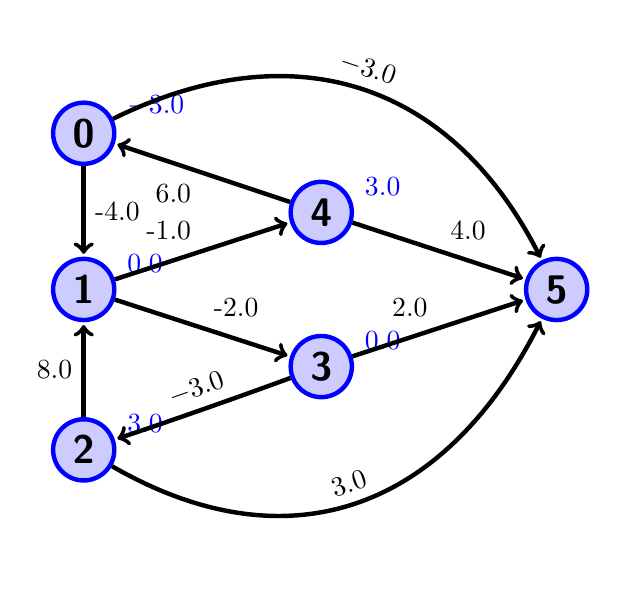
\begin{tikzpicture}[shorten >=1pt, auto, node distance=3cm, ultra thick,
        node_style/.style={circle,draw=blue,fill=blue!20!,font=\sffamily\Large\bfseries},
        edge_node_style/.style={draw=none,fill=none,midway,sloped},
        selected_node_style/.style={circle,draw=blue,fill=yellow!20!,font=\sffamily\Large\bfseries},
        edge_style/.style={draw=black, ultra thick,->},
        selected_edge_style/.style={draw=yellow, ultra thick,->}]
        \tikzset{quadratic bezier/.style={ to path={(\tikztostart) .. controls($#1!1/3!(\tikztostart)$) and ($#1!1/3!(\tikztotarget)$).. (\tikztotarget)}}}
        
        \node [node_style,label={[text=blue]10:$-3.0$}](n1) at (3.471,-1.527) {0};
        \node [node_style,label={[text=blue]10:$0.0$}](n2) at (3.471,-3.511) {1};
        \node [node_style,label={[text=blue]10:$3.0$}](n3) at (3.471,-5.548) {2};
        \node [node_style,label={[text=blue]10:$0.0$}](n4) at (6.488,-4.49) {3};
        \node [node_style,label={[text=blue]10:$3.0$}](n5) at (6.488,-2.532) {4};
        \node [node_style,label={[text=blue]10:$$}](n6) at (9.478,-3.511) {5};\draw [edge_style] (n2) to[edge label=-1.0] (n5);
            \coordinate (crtl2)  at (7.473,0.442);
                        \draw [edge_style] (n1) .. controls($(crtl2)!1/3!(n1)$) and ($(crtl2)!1/3!(n6)$).. node [edge_node_style] {$-3.0$} (n6);
                    \coordinate (crtl3)  at (7.324,-7.771);
                        \draw [edge_style] (n3) .. controls($(crtl3)!1/3!(n3)$) and ($(crtl3)!1/3!(n6)$).. node [edge_node_style] {$3.0$} (n6);
                    \coordinate (crtl4)  at (5.003,-5.039);
                        \draw [edge_style] (n4) .. controls($(crtl4)!1/3!(n4)$) and ($(crtl4)!1/3!(n3)$).. node [edge_node_style] {$-3.0$} (n3);
                    \draw [edge_style] (n5) to[edge label=4.0] (n6);
            \draw [edge_style] (n5) to[edge label=6.0] (n1);
            \draw [edge_style] (n2) to[edge label=-2.0] (n4);
            \draw [edge_style] (n4) to[edge label=2.0] (n6);
            \draw [edge_style] (n3) to[edge label=8.0] (n2);
            \draw [edge_style] (n1) to[edge label=-4.0] (n2);
            
        \end{tikzpicture}
    
            \end{center}
            \end{frame}
        
            \begin{frame}
            \frametitle{Bellman-Ford Algorithm : Iteration 3 }
            \begin{center}
            
        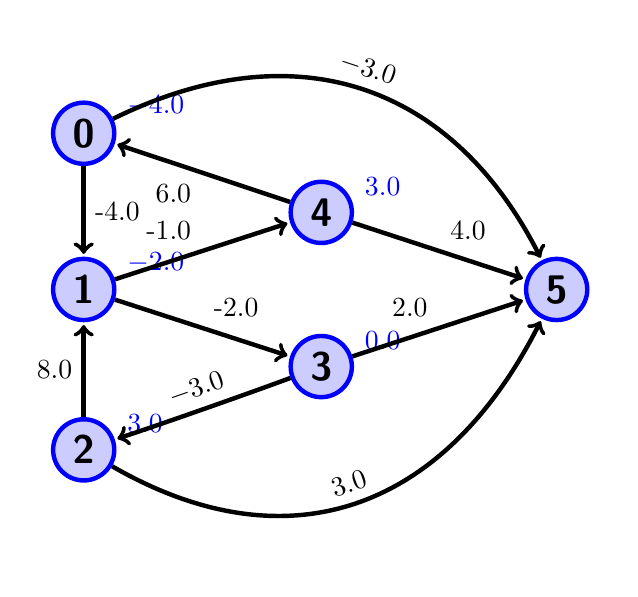
\begin{tikzpicture}[shorten >=1pt, auto, node distance=3cm, ultra thick,
        node_style/.style={circle,draw=blue,fill=blue!20!,font=\sffamily\Large\bfseries},
        edge_node_style/.style={draw=none,fill=none,midway,sloped},
        selected_node_style/.style={circle,draw=blue,fill=yellow!20!,font=\sffamily\Large\bfseries},
        edge_style/.style={draw=black, ultra thick,->},
        selected_edge_style/.style={draw=yellow, ultra thick,->}]
        \tikzset{quadratic bezier/.style={ to path={(\tikztostart) .. controls($#1!1/3!(\tikztostart)$) and ($#1!1/3!(\tikztotarget)$).. (\tikztotarget)}}}
        
        \node [node_style,label={[text=blue]10:$-4.0$}](n1) at (3.471,-1.527) {0};
        \node [node_style,label={[text=blue]10:$-2.0$}](n2) at (3.471,-3.511) {1};
        \node [node_style,label={[text=blue]10:$3.0$}](n3) at (3.471,-5.548) {2};
        \node [node_style,label={[text=blue]10:$0.0$}](n4) at (6.488,-4.49) {3};
        \node [node_style,label={[text=blue]10:$3.0$}](n5) at (6.488,-2.532) {4};
        \node [node_style,label={[text=blue]10:$$}](n6) at (9.478,-3.511) {5};\draw [edge_style] (n2) to[edge label=-1.0] (n5);
            \coordinate (crtl2)  at (7.473,0.442);
                        \draw [edge_style] (n1) .. controls($(crtl2)!1/3!(n1)$) and ($(crtl2)!1/3!(n6)$).. node [edge_node_style] {$-3.0$} (n6);
                    \coordinate (crtl3)  at (7.324,-7.771);
                        \draw [edge_style] (n3) .. controls($(crtl3)!1/3!(n3)$) and ($(crtl3)!1/3!(n6)$).. node [edge_node_style] {$3.0$} (n6);
                    \coordinate (crtl4)  at (5.003,-5.039);
                        \draw [edge_style] (n4) .. controls($(crtl4)!1/3!(n4)$) and ($(crtl4)!1/3!(n3)$).. node [edge_node_style] {$-3.0$} (n3);
                    \draw [edge_style] (n5) to[edge label=4.0] (n6);
            \draw [edge_style] (n5) to[edge label=6.0] (n1);
            \draw [edge_style] (n2) to[edge label=-2.0] (n4);
            \draw [edge_style] (n4) to[edge label=2.0] (n6);
            \draw [edge_style] (n3) to[edge label=8.0] (n2);
            \draw [edge_style] (n1) to[edge label=-4.0] (n2);
            
        \end{tikzpicture}
    
            \end{center}
            \end{frame}
        
            \begin{frame}
            \frametitle{Bellman-Ford Algorithm : Iteration 4 }
            \begin{center}
            
        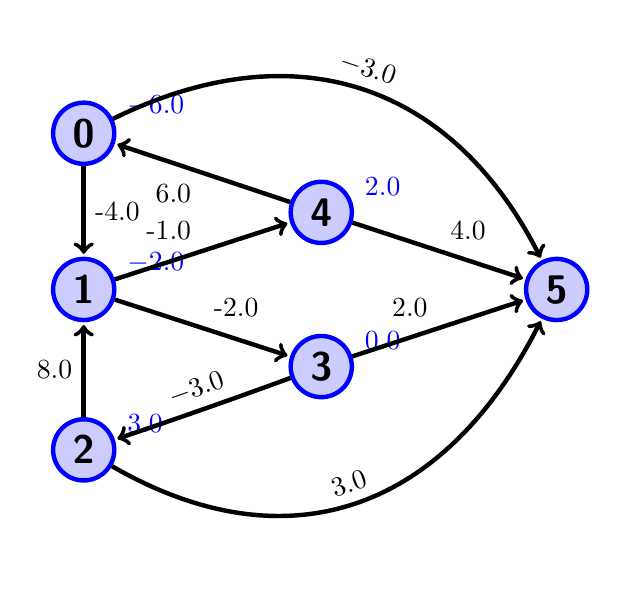
\begin{tikzpicture}[shorten >=1pt, auto, node distance=3cm, ultra thick,
        node_style/.style={circle,draw=blue,fill=blue!20!,font=\sffamily\Large\bfseries},
        edge_node_style/.style={draw=none,fill=none,midway,sloped},
        selected_node_style/.style={circle,draw=blue,fill=yellow!20!,font=\sffamily\Large\bfseries},
        edge_style/.style={draw=black, ultra thick,->},
        selected_edge_style/.style={draw=yellow, ultra thick,->}]
        \tikzset{quadratic bezier/.style={ to path={(\tikztostart) .. controls($#1!1/3!(\tikztostart)$) and ($#1!1/3!(\tikztotarget)$).. (\tikztotarget)}}}
        
        \node [node_style,label={[text=blue]10:$-6.0$}](n1) at (3.471,-1.527) {0};
        \node [node_style,label={[text=blue]10:$-2.0$}](n2) at (3.471,-3.511) {1};
        \node [node_style,label={[text=blue]10:$3.0$}](n3) at (3.471,-5.548) {2};
        \node [node_style,label={[text=blue]10:$0.0$}](n4) at (6.488,-4.49) {3};
        \node [node_style,label={[text=blue]10:$2.0$}](n5) at (6.488,-2.532) {4};
        \node [node_style,label={[text=blue]10:$$}](n6) at (9.478,-3.511) {5};\draw [edge_style] (n2) to[edge label=-1.0] (n5);
            \coordinate (crtl2)  at (7.473,0.442);
                        \draw [edge_style] (n1) .. controls($(crtl2)!1/3!(n1)$) and ($(crtl2)!1/3!(n6)$).. node [edge_node_style] {$-3.0$} (n6);
                    \coordinate (crtl3)  at (7.324,-7.771);
                        \draw [edge_style] (n3) .. controls($(crtl3)!1/3!(n3)$) and ($(crtl3)!1/3!(n6)$).. node [edge_node_style] {$3.0$} (n6);
                    \coordinate (crtl4)  at (5.003,-5.039);
                        \draw [edge_style] (n4) .. controls($(crtl4)!1/3!(n4)$) and ($(crtl4)!1/3!(n3)$).. node [edge_node_style] {$-3.0$} (n3);
                    \draw [edge_style] (n5) to[edge label=4.0] (n6);
            \draw [edge_style] (n5) to[edge label=6.0] (n1);
            \draw [edge_style] (n2) to[edge label=-2.0] (n4);
            \draw [edge_style] (n4) to[edge label=2.0] (n6);
            \draw [edge_style] (n3) to[edge label=8.0] (n2);
            \draw [edge_style] (n1) to[edge label=-4.0] (n2);
            
        \end{tikzpicture}
    
            \end{center}
            \end{frame}
        
            \begin{frame}
            \frametitle{Bellman-Ford Algorithm : Iteration 5 }
            \begin{center}
            
        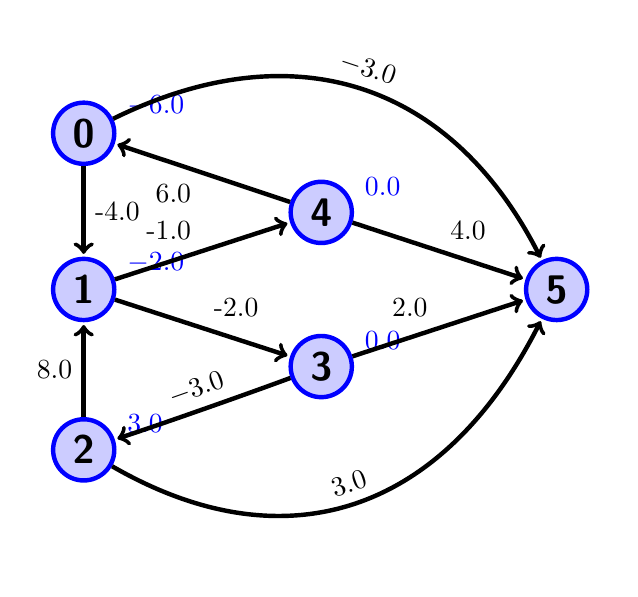
\begin{tikzpicture}[shorten >=1pt, auto, node distance=3cm, ultra thick,
        node_style/.style={circle,draw=blue,fill=blue!20!,font=\sffamily\Large\bfseries},
        edge_node_style/.style={draw=none,fill=none,midway,sloped},
        selected_node_style/.style={circle,draw=blue,fill=yellow!20!,font=\sffamily\Large\bfseries},
        edge_style/.style={draw=black, ultra thick,->},
        selected_edge_style/.style={draw=yellow, ultra thick,->}]
        \tikzset{quadratic bezier/.style={ to path={(\tikztostart) .. controls($#1!1/3!(\tikztostart)$) and ($#1!1/3!(\tikztotarget)$).. (\tikztotarget)}}}
        
        \node [node_style,label={[text=blue]10:$-6.0$}](n1) at (3.471,-1.527) {0};
        \node [node_style,label={[text=blue]10:$-2.0$}](n2) at (3.471,-3.511) {1};
        \node [node_style,label={[text=blue]10:$3.0$}](n3) at (3.471,-5.548) {2};
        \node [node_style,label={[text=blue]10:$0.0$}](n4) at (6.488,-4.49) {3};
        \node [node_style,label={[text=blue]10:$0.0$}](n5) at (6.488,-2.532) {4};
        \node [node_style,label={[text=blue]10:$$}](n6) at (9.478,-3.511) {5};\draw [edge_style] (n2) to[edge label=-1.0] (n5);
            \coordinate (crtl2)  at (7.473,0.442);
                        \draw [edge_style] (n1) .. controls($(crtl2)!1/3!(n1)$) and ($(crtl2)!1/3!(n6)$).. node [edge_node_style] {$-3.0$} (n6);
                    \coordinate (crtl3)  at (7.324,-7.771);
                        \draw [edge_style] (n3) .. controls($(crtl3)!1/3!(n3)$) and ($(crtl3)!1/3!(n6)$).. node [edge_node_style] {$3.0$} (n6);
                    \coordinate (crtl4)  at (5.003,-5.039);
                        \draw [edge_style] (n4) .. controls($(crtl4)!1/3!(n4)$) and ($(crtl4)!1/3!(n3)$).. node [edge_node_style] {$-3.0$} (n3);
                    \draw [edge_style] (n5) to[edge label=4.0] (n6);
            \draw [edge_style] (n5) to[edge label=6.0] (n1);
            \draw [edge_style] (n2) to[edge label=-2.0] (n4);
            \draw [edge_style] (n4) to[edge label=2.0] (n6);
            \draw [edge_style] (n3) to[edge label=8.0] (n2);
            \draw [edge_style] (n1) to[edge label=-4.0] (n2);
            
        \end{tikzpicture}
    
            \end{center}
            \end{frame}
        
        \end{document}
    
